%%%%%%%%%%%%%%%%%%%%%%%%%%%%%%%%%%%%%%%%%%%%%%%%%%%%%%%%%%%%%%%%%%%%%%%%%%%%%%%%
\chapter{Prototype}
\label{sec:implement}
%%%%%%%%%%%%%%%%%%%%%%%%%%%%%%%%%%%%%%%%%%%%%%%%%%%%%%%%%%%%%%%%%%%%%%%%%%%%%%%%

We prototyped Trusted Capsules on a LeMaker HiKey development
board~\cite{hikey}. It has an octa-core ARM Cortex-A53 processor, 2~GB
of RAM, 8~GB of flash storage. and it comes with TrustZone unlocked,
thereby allowing us to control what OS runs on the TEE. We use Linaro
OP-TEE OS (version 3.3) in TrustZone and a HiKey Debian OS (based on
Linux 4.4.15) in the normal world. We modified the OP-TEE OS to
implement several missing {\tt libc} functions (such as {\tt atoi} and
{\tt strcmp}). As the HiKey board does not have a GPS receiver, we
mocked a GPS device that returns predefined longitude and latitude
values.

Capsules are encrypted with 128-bit AES. We consider the distribution
of keys required to decrypt capsules outside the scope of this paper.

Our data monitor is written in C and consists of about 6.2K SLOC: the
policy execution engine, which runs within the TEE, has about 4.2K
SLOC while the normal world framework has 2K.

%%%%%%%%%%%%%%%%%%%%%%%%%%%%%%%%%%%%%%%%%%%%%%%%%%%%%%%%%%%%%%%%%%%%%%%%%%%%%%%%%%%%%
\subsection{Prototype Evolution}\label{sub:proto-prototype}
%%%%%%%%%%%%%%%%%%%%%%%%%%%%%%%%%%%%%%%%%%%%%%%%%%%%%%%%%%%%%%%%%%%%%%%%%%%%%%%%%%%%%

The system design and the prototype evaluated in this paper has
evolved from a previous design of the system. This prior system
(``version-0'') had the ambitious goal of evaluating a Lua-based
policy in TEE on all intercepted file I/O system calls on a capsule
file: \texttt{open}, \texttt{close}, \texttt{read}, \texttt{write},
and \texttt{lseek}. As well, Version-0 revealed \emph{chunks} of the
file to normal world applications, rather than decrypting and
revealing the entire file contents on \texttt{open}. Version-0 was not
based on FUSE, but it used a custom system call interceptor in the
normal world OS. This interceptor worked in a manner similar to the
FUSE filesystem in our current design

Version-0 prototype was mature and stable, but had to be abandoned
because of unacceptable application slowdown. This was due to the
invasive nature of the system call handler that slowed down the
behaviour of most applications that open and close many files at
start-up. 

More concretely, the time to open a small document under a no-op
policy with FUSE on our hardware is 24ms, %\iv{.5s}
while the latency in Version-0 was 1.2s. %\iv{5s}. 
This is a speed-up of 50x over Version-0.

%By contrast, in our current prototype the
%latency is \iv{1s}, which is a speed up of \iv{5x} over Version-0. 

The latency and throughput gap dramatically increased for large and
complex file types, such as PDF JPEG. This can be observed in the raw
video footage for several use-cases in Version-0 of the system:
\url{https://goo.gl/SiBEJB}.

We note that while overhead in Version-0 was significantly better at
the application layer as compared to the system call layer,
nevertheless, the cost was prohibitive and was tightly connected to
the policy being used.
%
%% %% For various data types, a null
%% %% policy had much less significant or almost imperceivable impact to
%% %% usability at the application level. However, 
%% our use-case policies, some of which contained expensive policy checks
%% (e.g., access to state storage or going over the network to talk to
%% the policy coordinator) on frequent operations such as read or write,
%% resulted in noticeable performance degradation.
%
For example, our MP4 video played smoothly with a null policy in VLC
(which did not interact with the trusted capsule server), but degraded
to extreme jitter once we added a policy that reported actions to a
policy coordinator and accessed secure storage for every read
operation. This effect was particularly acute for the PDF reader,
which repeatedly read the data in small chunks frequently and even
when the user was idle. Each read by the PDF incurred the cost of a
single round-trip to the trusted capsule server, requiring on average
5ms each. 

Our experiences with Version-0 of the Trusted Capsules prototype have
been our guiding principle in making our current system perform
better.
%
Our benchmarking results (presented in the next Section) indicate which
the current Trusted Capsules design, that evaluates policy exclusively
on \texttt{open} and \texttt{close} calls, strikes a better trade-off
between security and performance.


%% Our prototype
%% supports the following composable policy actions:

%% \begin{itemize}

%% %\item Allowing or denying the operation on the trusted capsule.

%% \item Allowing or denying the capsule to be opened or modified based on various
%%   signals such as location, time, or device identity.

%% % \item Reporting the operation, location, time, role-identity of the
%% %   device to a global policy coordinator.

%% \item Logging capsule accesses and reporting them to a remote server.

%% %\item Initializing or modifying persistent state (e.g., counter).

%% \item Initializing or modifying persistent capsule metadata (e.g., counter).

%% % \item Performing byte-based or keyword-based redaction that partially
%% %   discloses trusted capsule data. %A data-type specific pre-processor
%% %   %can be used to generate the byte offsets.

%% \item Performing byte-based or keyword-based redaction that partially discloses
%%   trusted capsule data. \ar{Table~\ref{Tbl:lua_ext} doesn't list the API to
%%     perform keyword-based redaction.} \pu{all redaction is based on byte offsets. the keyword search happens in lua and then the byte offsets are passed to the C API. How should I phrase this then?}

%% \item Hard access revocation by deleting the capsule, triggered
%%   locally or remotely; and, gradual access revocation based on evolving policy decisions that are adaptive to context of access - for example, total number of accesses, passage of time, policy updation, etc.
%%   %soft revocation by arbitrarily changing
%%   %the policy. 
%%   \ar{What's soft revocation?}\pu{Check}

%% % \item Prevent declassification through the network or file system.


%% %\item Registering a callback -- to place a deterministic real-time bound on when a policy is re-evaluated
%% %\item Killing a running process

%% \end{itemize}


%% %%%%%%%%%%%%%%%%%%%%%%%%%%%%%%%%%%%%%%%%%%%%%%%%%%%%%%%%%%%%%%%%%%%%%%%%%%%%%%%%%%%%%
%% \subsection{Prototype Limitations}\label{sub:proto-limitations}
%% %%%%%%%%%%%%%%%%%%%%%%%%%%%%%%%%%%%%%%%%%%%%%%%%%%%%%%%%%%%%%%%%%%%%%%%%%%%%%%%%%%%%%

%% %% In this section we list the limitations that bound the current
%% %% prototype from realizing the fulll vision of the Trusted Capsule model
%% %% of data protection. Here we note some design and implementation
%% %% limitations.

%% FUSE can interpose on only the file I/O system calls that are directed
%% to a FUSE serviced mountpoint. This poses some challenges in making
%% Trusted Capsules work seamlessly with an unmodified application. We assume 

%% There is no way for the FUSE filesystem code to identify when a
%% process that had been issuing IO to the mountpoint dies. The
%% implication of this fact for the prototype is that there is no good
%% and atomic way to delete the shadow file on the termination of the
%% process. The prototype handles this by setting up a background process
%% that monitors if the process that had accessed the mountpoint has
%% terminated.

%% The stock configuration for the TrustZone memory partitions makes the
%% Secure World a very memory constrained environment. The memory that is
%% available in the secure world is only 10 MB, and that needs to host
%% the Secure OS as well as any trusted application code that must run in
%% Trustzone.

%% This limitation hits our prototype particularly badly. In the current
%% prototype, we send a copy of the entire file to TrustZone to
%% decrypt. Since there are severe restrictions on the amount of memory
%% available in TrustZone, we are unwittingly bounded on the maximum file
%% size that can be processed as a capsule.

%% % Linaro OP-TEE recently included dynamic shared memory in their
%% % Secure OS, but to access those features, one has to have a higher
%% % kernel version than what gets shipped with the stock Debian OS
%% % rootfs image. Higher Linux kernel versions have known problems with
%% % the HDMI drivers, which causes the Linux kernel to panic when a
%% % monitor is plugged in.

%% The implementation has a limitation that it needs to create copies of
%% the data buffers to process each part of the capsule. This creates
%% more memory pressure in an already resource constrained environment.


%% It does, however, still remains a true manifestation of the
%% idea of Trusted Capsules and operates under a similar threat model.

%% In Section ~\ref{sec:eval}, we evaluate our current prototype, and
%% provide a brief description of the performance improvements from the
%% design change.  We compare the performance of our prototype against
%% the prior prototype and demonstrate that the current prototype is
%% faster.  \pu{write about how the old prototype provides us with
%%   compatibility that we haven't yet achieved with the current
%%   prototype.}  \pu{There has to be a better way of referencing them
%%   other than saying old and new/current prototype.}

%%%%%%%%%%


% %%%%%%%%%%%%%%%%%%%%%
%% \begin{figure}
%%   \centering
%%   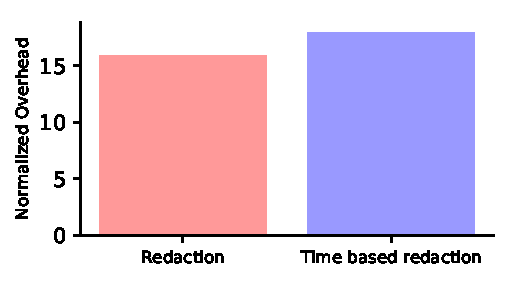
\includegraphics[width=8cm,height=4cm]{fig/policy_latencies.pdf}  
%%   \caption{Normalized latency of servicing an \texttt{open} for different policies with respect to the latency to service a null-policy capsule open request. }
%%   \label{fig:policy_latency}
%% \end{figure}
% %%%%%%%%%%%%%%%%%%%%%/


%% To identify the impact on applications operating on trusted capsules,
%% we look back and reference the work we had done for the first
%% generation prototype. Our experiences when creating the first
%% generation of the prototype have been our guiding principle for making
%% the system perform better. We present here the perceived latencies for
%% applications that operate on capsules while performing some
%% non-trivial tasks. \footnote{The reader is reminded that the following
%%   results are based on the first generation prototype which is based
%%   on the older system that used system call interceptor mechanism as
%%   described in ~\ref{sub:proto-prototype}}

%% We measured the impact under three different conditions: with an empty
%% null policy, with our use case policies, and without trusted capsules
%% (as a baseline). Some of our use case policies, such as those on the
%% PDF and JPEG, required a trusted capsule server in order to fetch
%% remote state and report logged information. For all data type
%% use-cases, we implemented use-case policies described in
%% Section~\ref{sec:new-policies}, except for redactions on PDF
%% documents, which required knowing PDF's binary format.

%% We used a Canon Rebel II DSLR to film certain interactions between the trusted capsule and applications. We then measured the latency between
%% the start of an action (e.g. open a document) and when the action is
%% completed. We filmed at 60 FPS and used the difference in timestamps
%% to calculate the application latency. We present our results in
%% Table~\ref{Tbl-Macro-performance} and provide the raw footage online:
%% \url{https://goo.gl/SiBEJB}.

%%%%%%%%%%



% We used Linaro OP-TEE OS (version 3.3) We modified the Linaro OP-TEE OS version
% 3.3 to be our TrustZone software stack and mounted a userspace filesystem in the
% normal world operating system that runs a custom Hikey Debian OS based on Linux
% kernel 4.4.15. \pu{check} In the FUSE filesystem, we intercept \textit{open} and
% \textit{close} system calls and redirect them to the secure world for decryption
% and encryption respectively. All accesses to non-capsule files proceed just like
% normal file operations on a FUSE mountpoint.

%We deployed ARM Trusted Firmware and a modified Linaro OP-TEE OS as our
%software stack in TrustZone.


%Our trusted capsule monitor in the normal world 
%consists of a modified Linaro OP-TEE supplicant and a modified Linaro OP-TEE Linux 
%Driver with our custom system call interceptor. The kernel components are deployed as
%Linux kernel module. 

% Our modifications to the OP-TEE OS in the secure world is limited to the
% implementation of a few missing \texttt{libc} functions like \texttt{atoi} and
% \texttt{strcmp}. These are minimal changes compared to the original OP-TEE code
% base.

%Our modifications to the OP-TEE components across the
%software stack in both worlds consist entirely of additional RPCs that 
%enable trusted capsule applications to access the file system and network
%directly. These modifications are minimal compared to the original OP-TEE
%code base. % Our implementation is based on OP-TEE 1.0. 


% twithin the OP-TEE Linux Driver that returns predefined longitude and latitude
% values.
%
% In the normal world, we run a pre-alpha release of a custom HiKey Debian OS
% based on Linux kernel 3.18.0.
%
% We used 128-bit AES and SHA-256 for encrypting and hashing trusted
% capsules.

% Our current implementation supports the following composable actions
% based on policy evaluation:

% \begin{itemize}

% \item Allowing or denying the operation on the trusted capsule.

% \item Initializing or modifying persistent state (e.g., counter).

% \item Performing byte-based or keyword-based redaction that partially
%   discloses trusted capsule data. %A data-type specific pre-processor
%   %can be used to generate the byte offsets.

% \item Reporting the operation, location, time, role-identity of the
%   device to a global policy coordinator.

% \item Hard access revocation by deleting the capsule, triggered
%   locally or remotely; and, soft revocation by arbitrarily changing
%   the policy.

% \item Prevent declassification through the network or file system.
% \pu{Review.}


%\item Registering a callback -- to place a deterministic real-time bound on when a policy is re-evaluated 
%\item Killing a running process 

%\end{itemize}

% In total, our trusted capsule application has 4.2K lines of
% non-comment C code and our filesystem code has 2K lines of
% non-comment C code.
